% 最终图1—6，按原比例缩放；插入后核对实际字号。

\begin{figure*}[t]
    \centering
    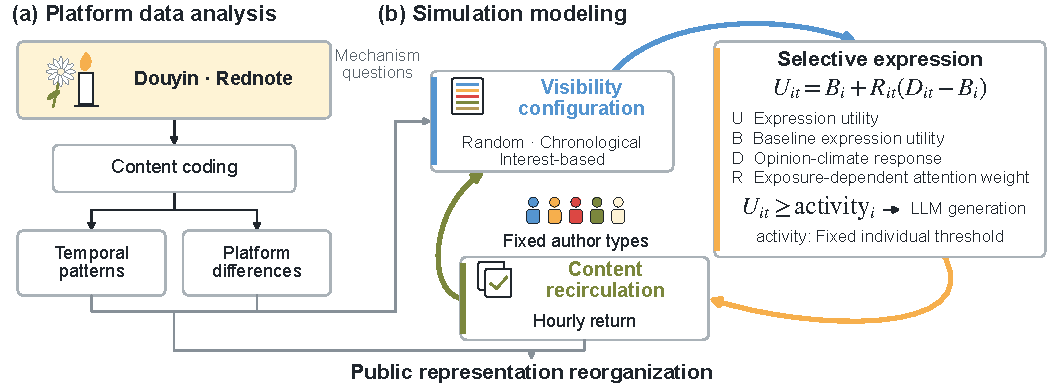
\includegraphics[width=\textwidth]{figure_01_framework.pdf}
    \caption{研究框架与表达效用驱动的表征重组机制。（a）平台内容分析识别公共讨论的时间变化与平台差异，为仿真提出机制问题；（b）在固定作者类型的条件下，比较随机、时序和兴趣三种策展制度，通过“可见性配置—选择性表达—内容回流”的循环考察表征重组。U、B、D、R分别表示表达效用、常态表达效用、意见气候响应和随累计同类接触衰减的注意力权重；下标i表示智能体，t表示行动时点。表达效用达到固定个体门槛activity\_i时触发大语言模型生成，成功发布的帖文在小时行动批次结束后回流候选池，成为后续批次的候选内容。两项研究共同解释公众人物身后公共表征的重组。}
    \label{fig:figure_01_framework}
\end{figure*}

\begin{figure*}[t]
    \centering
    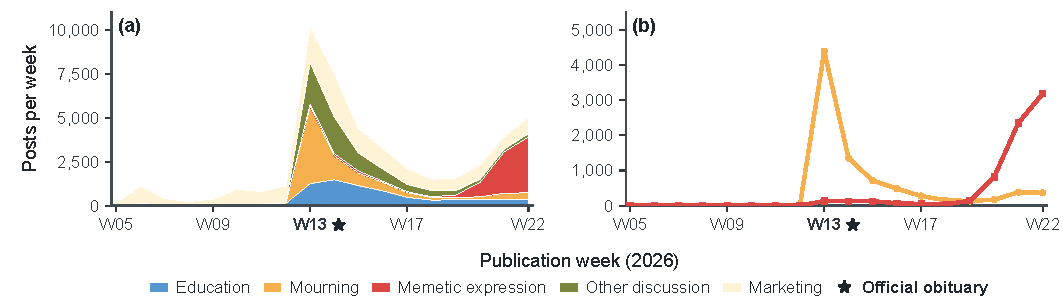
\includegraphics[width=\textwidth]{figure_02_observed_trends.pdf}
    \caption{两平台合并样本的内容数量及悼念、玩梗表达变化。（a）以堆积面积展示教育、悼念、玩梗、其他讨论和营销五类内容的周度数量，面积顶部为当周五类内容总量；（b）展示悼念与玩梗帖文的周度数量。五类分析样本共46,602条，横轴为2026年W05—W22，加粗W13与五角星标记官方讣告所在周。}
    \label{fig:figure_02_observed_trends}
\end{figure*}

\begin{figure*}[t]
    \centering
    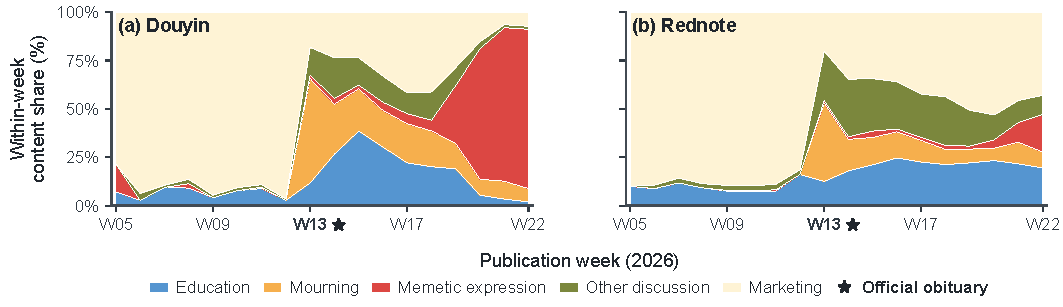
\includegraphics[width=\textwidth]{figure_03_observed_platforms.pdf}
    \caption{Douyin与Rednote的内容构成随时间的变化。（a）为Douyin，（b）为Rednote，堆积面积分别表示教育、悼念、玩梗、其他讨论和营销内容在当周五类内容中的比例。两平台五类样本分别为15,186条和31,416条，采用相同的比例轴与类别配色，每个平台每周的五类内容合计为100%。横轴为2026年W05—W22，加粗W13与五角星标记官方讣告所在周。}
    \label{fig:figure_03_observed_platforms}
\end{figure*}

\begin{figure*}[t]
    \centering
    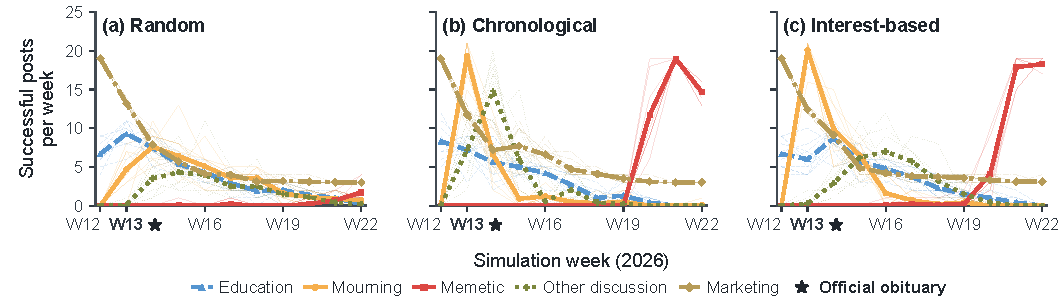
\includegraphics[width=\textwidth]{figure_04_simulated_trajectories.pdf}
    \caption{统一小时回流条件下三种策展制度的作者供给轨迹。（a）—（c）分别展示随机、时序和兴趣制度下五种固定作者类型在W12—W22的每周成功发帖数量。三面板采用相同的纵轴尺度与类别配色，细线表示各随机种子的轨迹，粗线表示10个种子的算术均值。每种制度包含10个种子，共30次运行；人口构成、外部输入和每周表达机会保持一致，生成帖在小时行动批次结束后入池。加粗W13与五角星标记官方讣告所在周。}
    \label{fig:figure_04_simulated_trajectories}
\end{figure*}

\begin{figure*}[t]
    \centering
    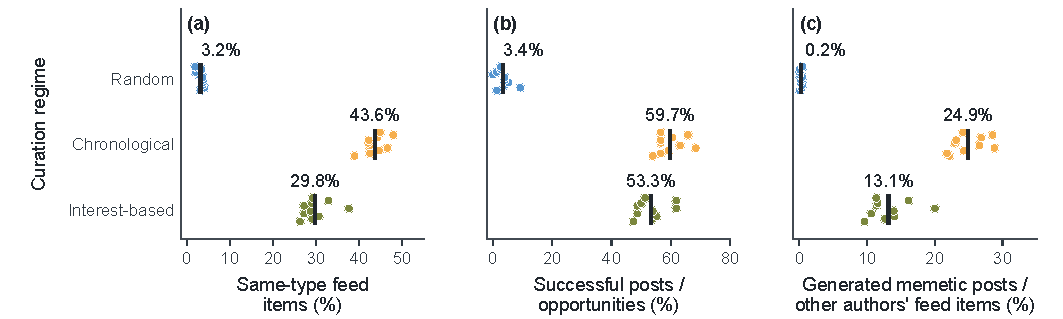
\includegraphics[width=\textwidth]{figure_05_feedback_exposure.pdf}
    \caption{统一小时回流条件下的同类接触、表达参与和生成帖跨群体再展示。（a）展示W19—W22玩梗型作者信息流中的同类内容比例；（b）展示该群体成功发帖数占表达机会的比例；（c）展示玩梗型作者生成帖占其他作者信息流全部展示的比例。三项指标在每次运行内分别以760条信息流展示、76次表达机会和3,240条信息流展示为分母计算。每种制度包含10个种子，共30次运行；散点表示各次运行，黑色短竖线及数字表示跨种子的算术均值。}
    \label{fig:figure_05_feedback_exposure}
\end{figure*}

\begin{figure*}[t]
    \centering
    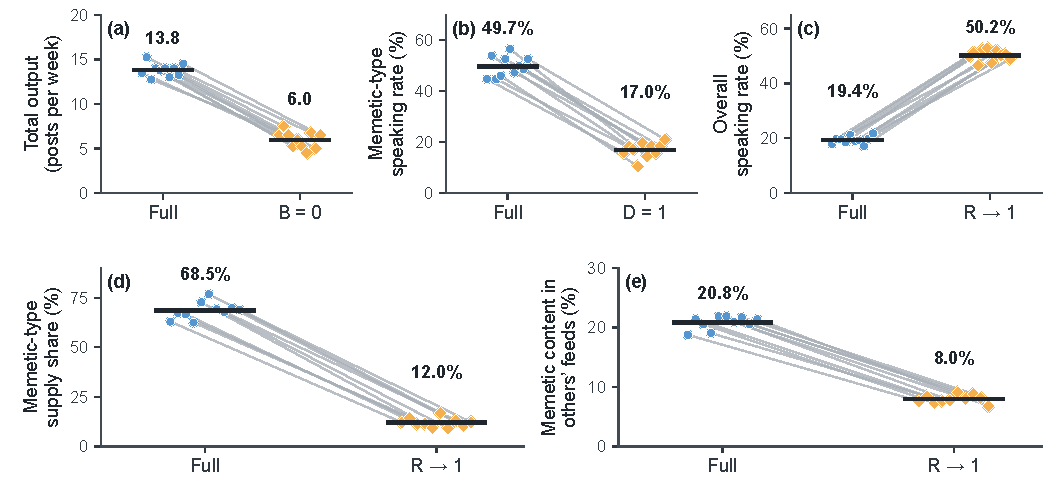
\includegraphics[width=\textwidth]{figure_06_bdr_ablation.pdf}
    \caption{表达组件干预对参与、供给及可见位置的影响。（a）比较完整模型与B=0条件下W19—W22的平均每周总供给；（b）比较完整模型与D=1条件下同期玩梗型作者的发言率；（c）比较完整模型与R → 1干预下W14—W18全体作者的发言率；（d）、（e）分别比较R → 1干预下W19—W22玩梗型作者的供给份额，以及其他作者信息流中玩梗内容的比例。各比较均采用原组件消融批次，在兴趣制度下进行，每种条件包含10个种子，完整模型与干预条件按种子配对，人口构成、外部输入和行动安排保持一致。散点表示各次运行，灰线连接同一种子的两个条件，黑色短横线及数字表示跨种子均值。发言率以相应群体的表达机会为分母，供给份额以全部智能体成功发帖为分母；（e）的玩梗内容包含外部帖与生成帖，分母为其他作者获得的信息流展示。}
    \label{fig:figure_06_bdr_ablation}
\end{figure*}
